\chapter{Aktivitäts- und Zustandsdiagramme}

\subsection{Rezept erstellen und veröffentlichen}
\begin{figure}[H]
	\centering
	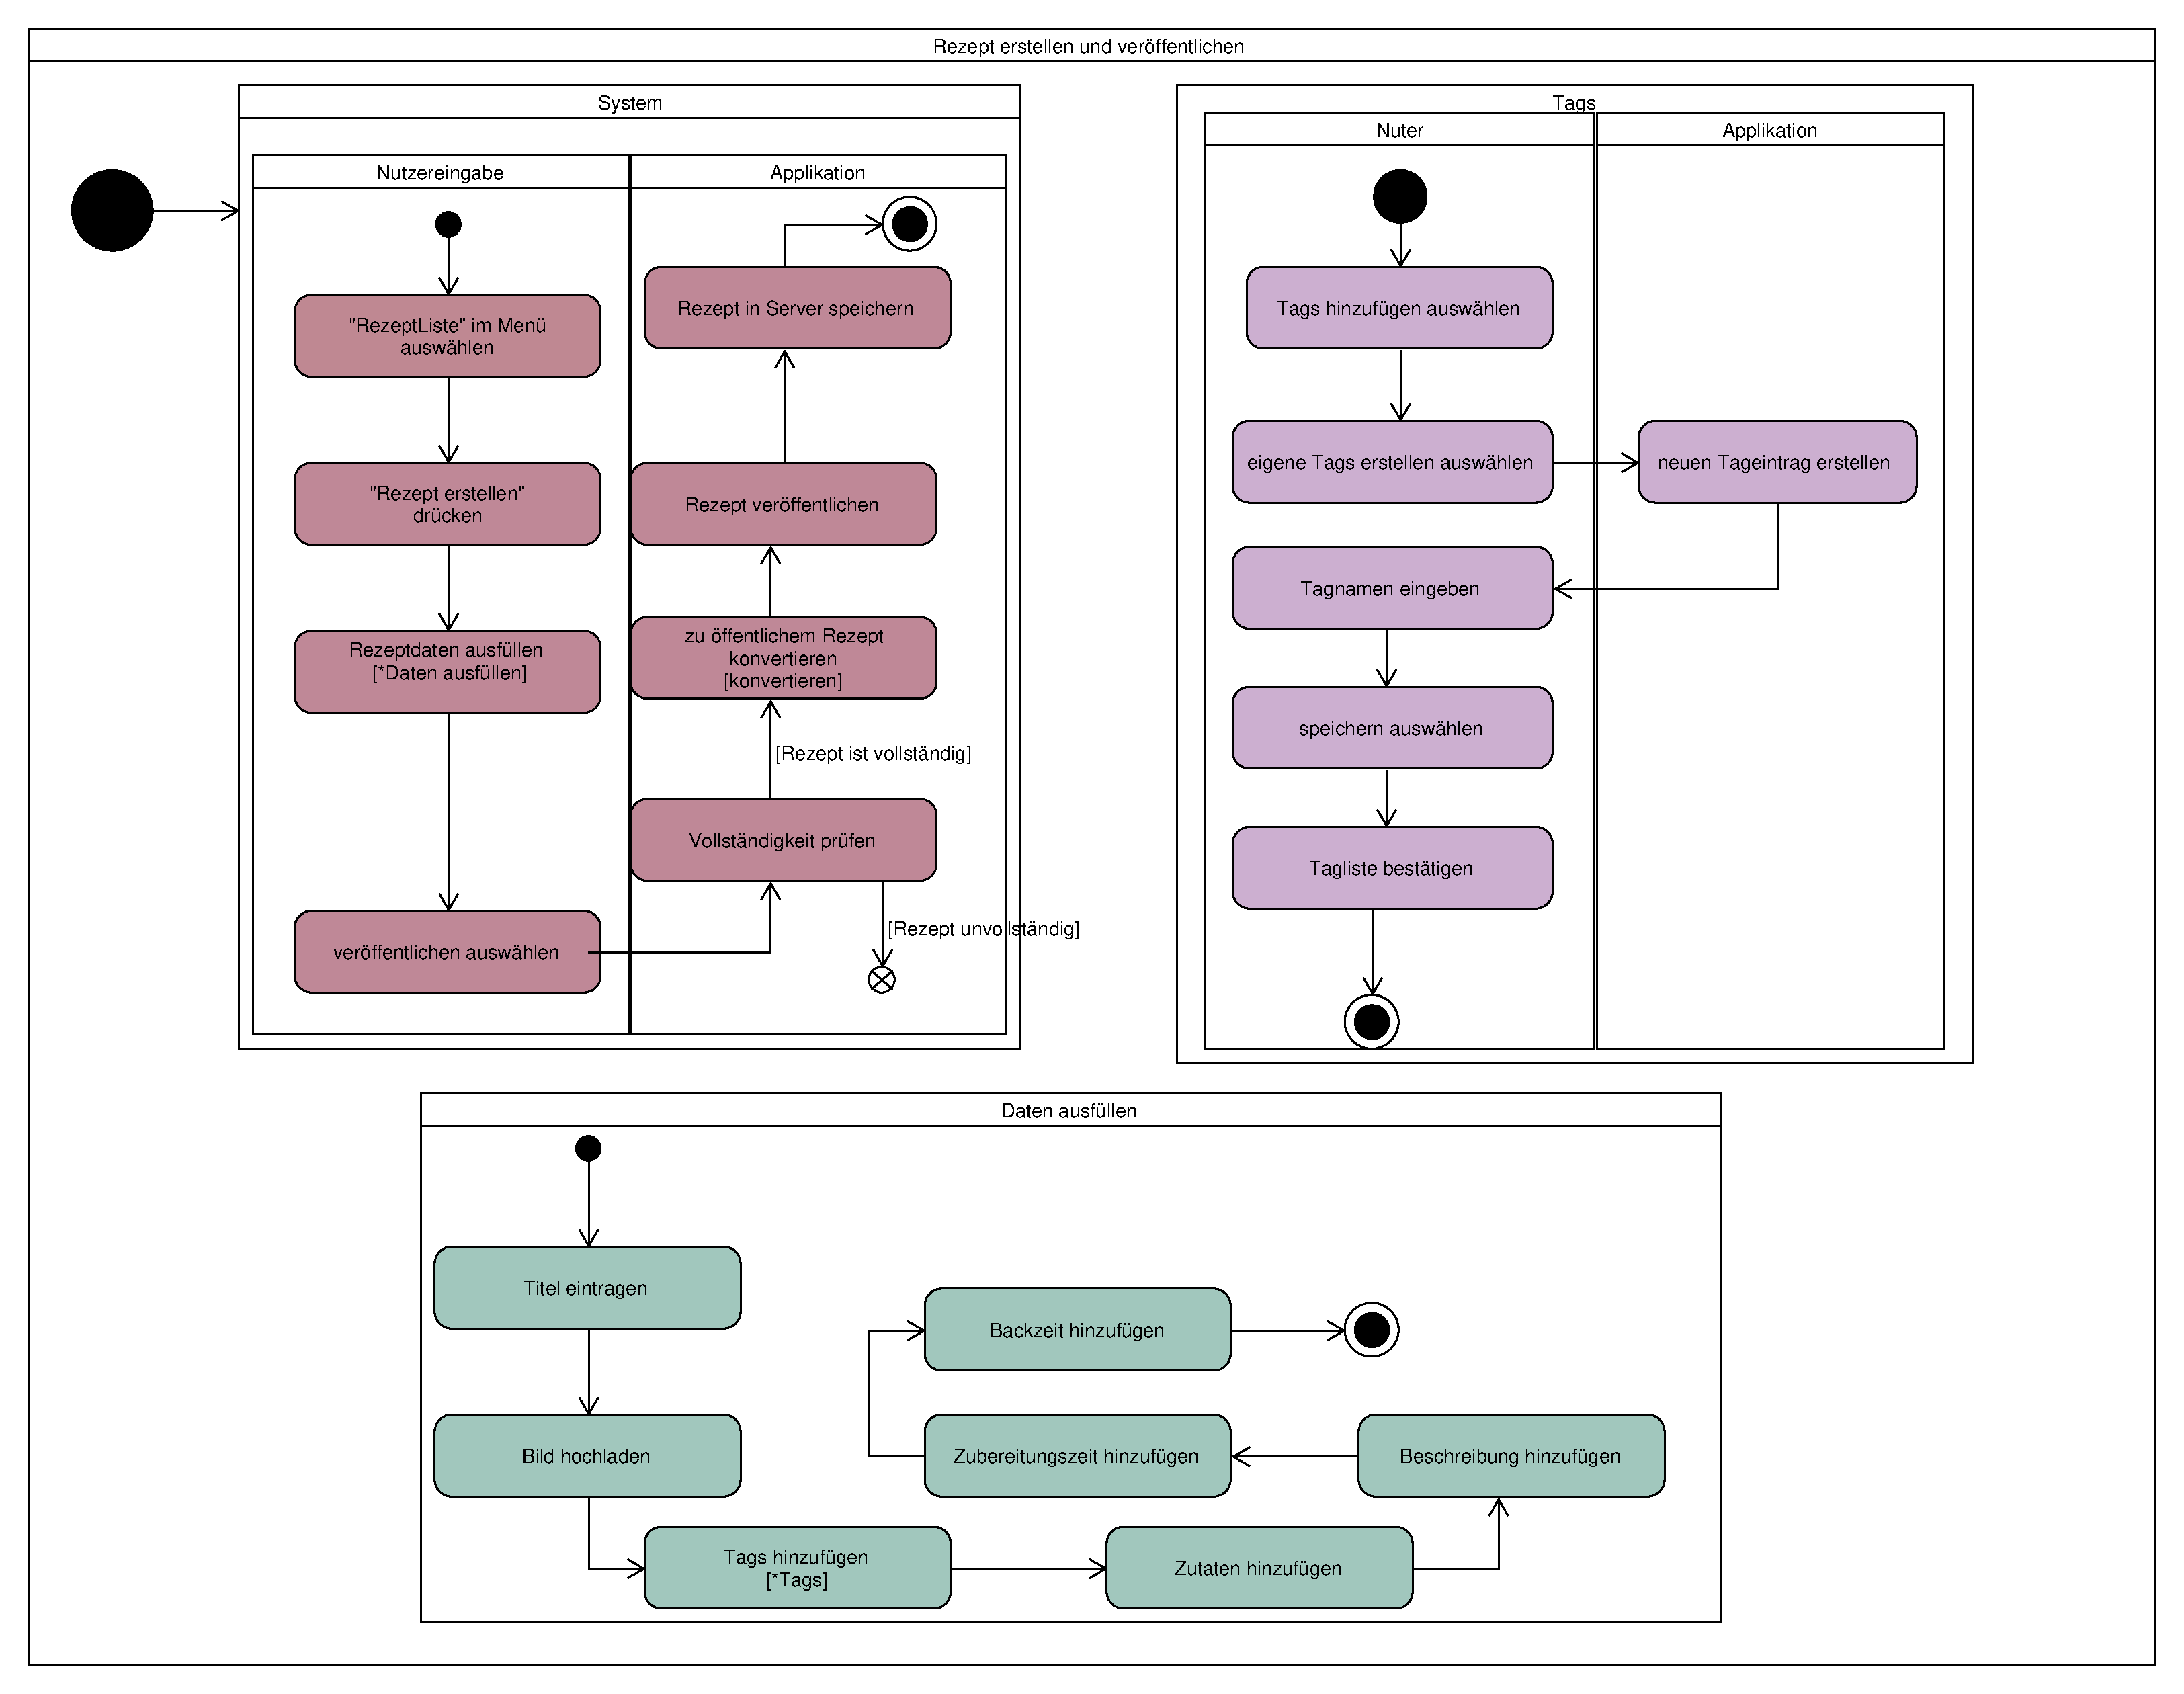
\includegraphics[width=\textwidth]{pics/dynamicDiagram/AktivitaetsdiagrammRezepterstellen.pdf}%
	\caption{Rezept erstellen und veröffentlichen}%
	\label{diagram}%
\end{figure}



Der Nutzer befindet sich in der Applikation und ist auf der Startseite. Nun will er ein Rezept erstellen und veröffentlichen. Dabei erstellt er noch ein eigenen neuen Tag. 


\subsubsection{System}
\begin{figure}[H]
	\centering
	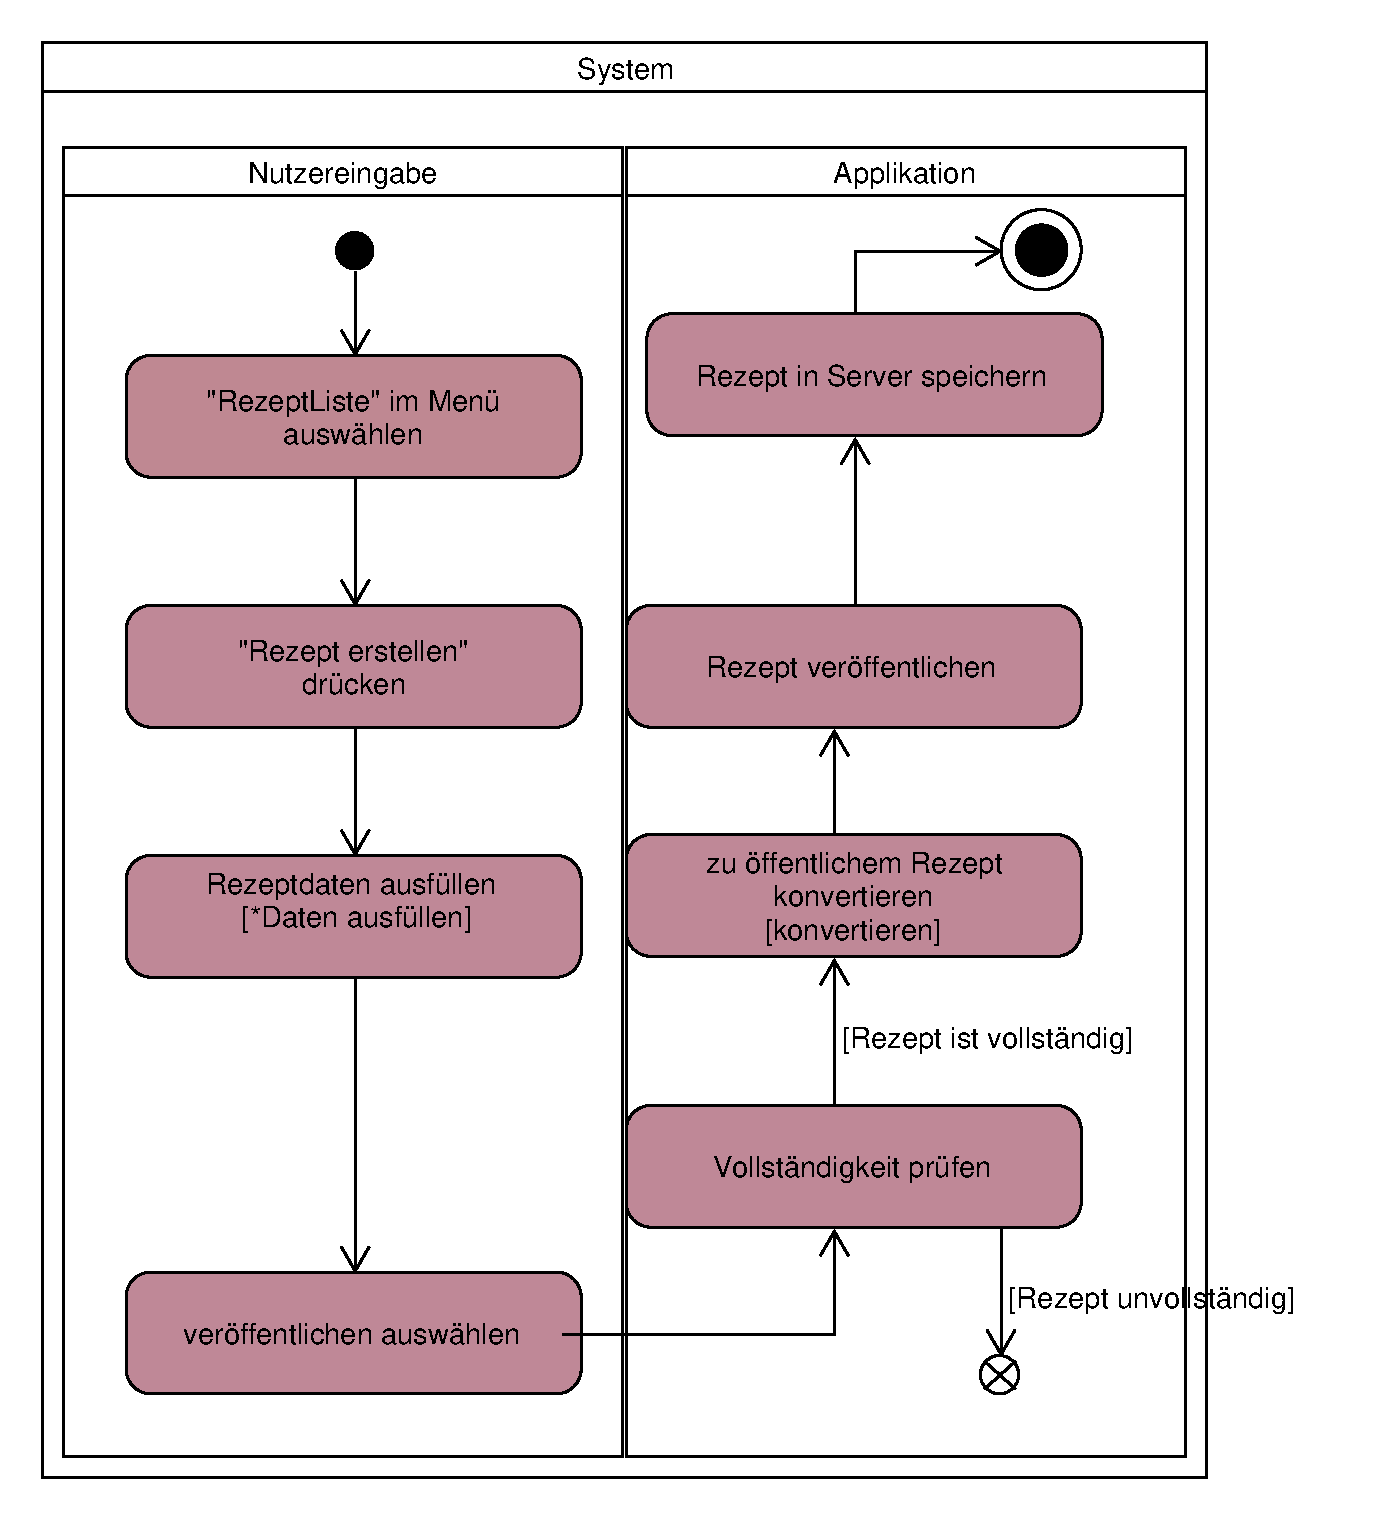
\includegraphics[width=\textwidth]{pics/dynamicDiagram/AktivitaetsdiagrammRezepterstellenSystem.pdf}%
	\caption{Rezept erstellen und veröffentlichen - System}%
	\label{diagram}%
\end{figure}


Der Nutzer befindet sich in der App Ansicht und wählt im Menü den Menüpunkt "Rezeptliste" aus. Dabei wechselt das Fragment und es wird die Liste an selbst erstellten, vollständigen und unvollständigen Rezepten angezeigt. Neben der Liste befindet sich ein Button mit der Aufschrift "Rezept erstellen", den der Nutzer auswählt. Es öffnet sich daraufhin ein neues Fenster, das ein Rezepteingabe Template anzeigt. (siehe Daten ausfüllen Aktivitätsdiagramm). 
Als der Nutzer die Daten ausgefüllt hat, wählt er die Option aus, sein Rezept öffentlich anzuzeigen. Daraufhin wird das Rezept im Hintergrund von einem Parser auf Vollständigkeit überprüft. Ist das Rezept nicht vollständig, wird das Rezept in der Rezeptliste gespeichert, zu der der Nutzer im nächsten Schritt geleitet wird. Ist das Rezept vollständig, wird es zu einem öffentlichen Rezept konvertiert (siehe konvertieren Aktivitätsdiagramm). Nachdem das Rezept in ein öffentliches konvertiert wurde wird es an den Server weitergeleitet, wo es in der Datenbank gespeichert wird.

\subsubsection{Daten}
\begin{figure}[H]
	\centering
	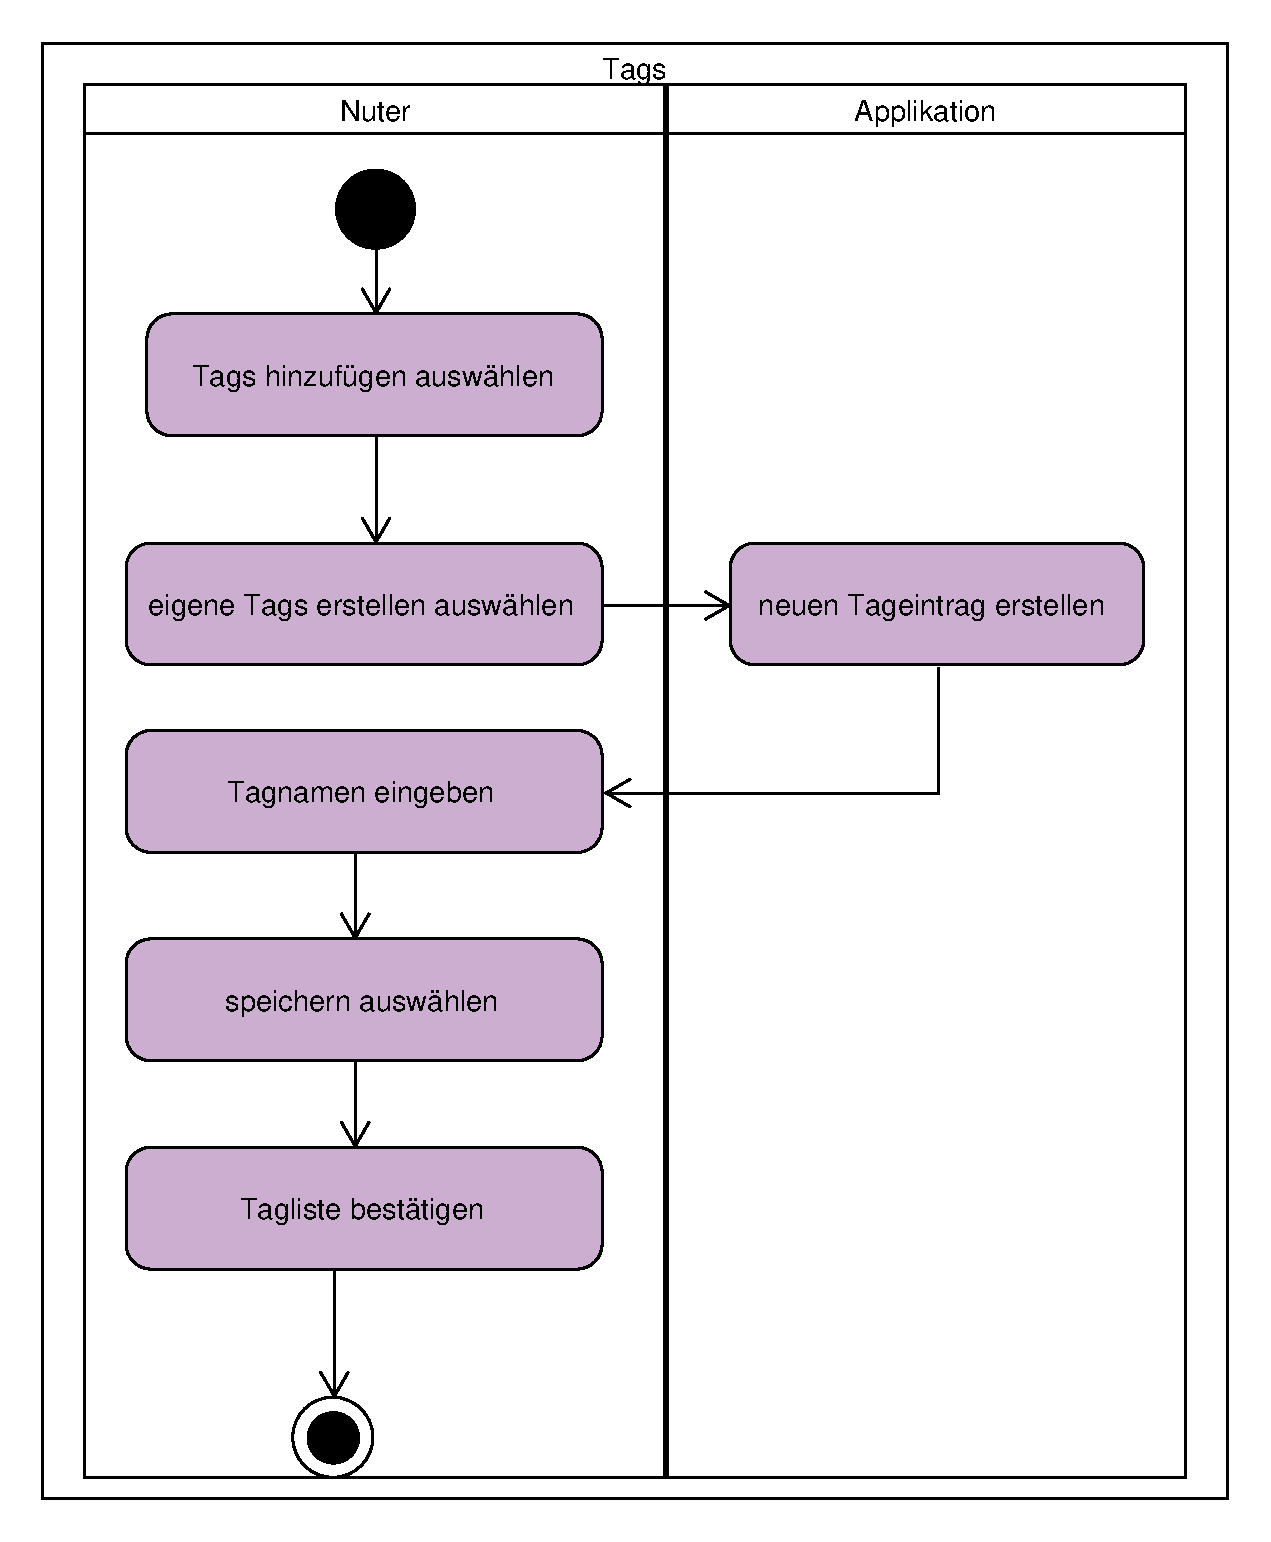
\includegraphics[width=\textwidth]{pics/dynamicDiagram/AktivitaetsdiagrammRezepterstellenDaten.pdf}%
	\caption{Rezept erstellen und veröffentlichen - Daten}%
	\label{diagram}%
\end{figure}


Der Nutzer befindet sich in der Rezept erstellen Ansicht, wo ihm ein Eingabe Template angeboten wird. Zuerst trägt er einen Titel ein und lädt ein Bild des Rezeptes hoch . Danach wählt er de Button "Tags hinzufügen" aus (siehe Tags hinzufügen Aktivitätsdiagramm). Daraufhin fügt er über eine Eingabe Zutaten zu dem Rezept hinzu. Nach den Zutaten beschreibt er die Zubereitung des Rezepts mit einem Freitext in dem dafür vorgesehenen Textfeld. Nun fügt er noch die Zubereitungs- und die Backzeit hinzu und hat damit seine Rezeptdaten vollständig ausgefüllt. 


\subsubsection{Tags}
\begin{figure}[H]
	\centering
	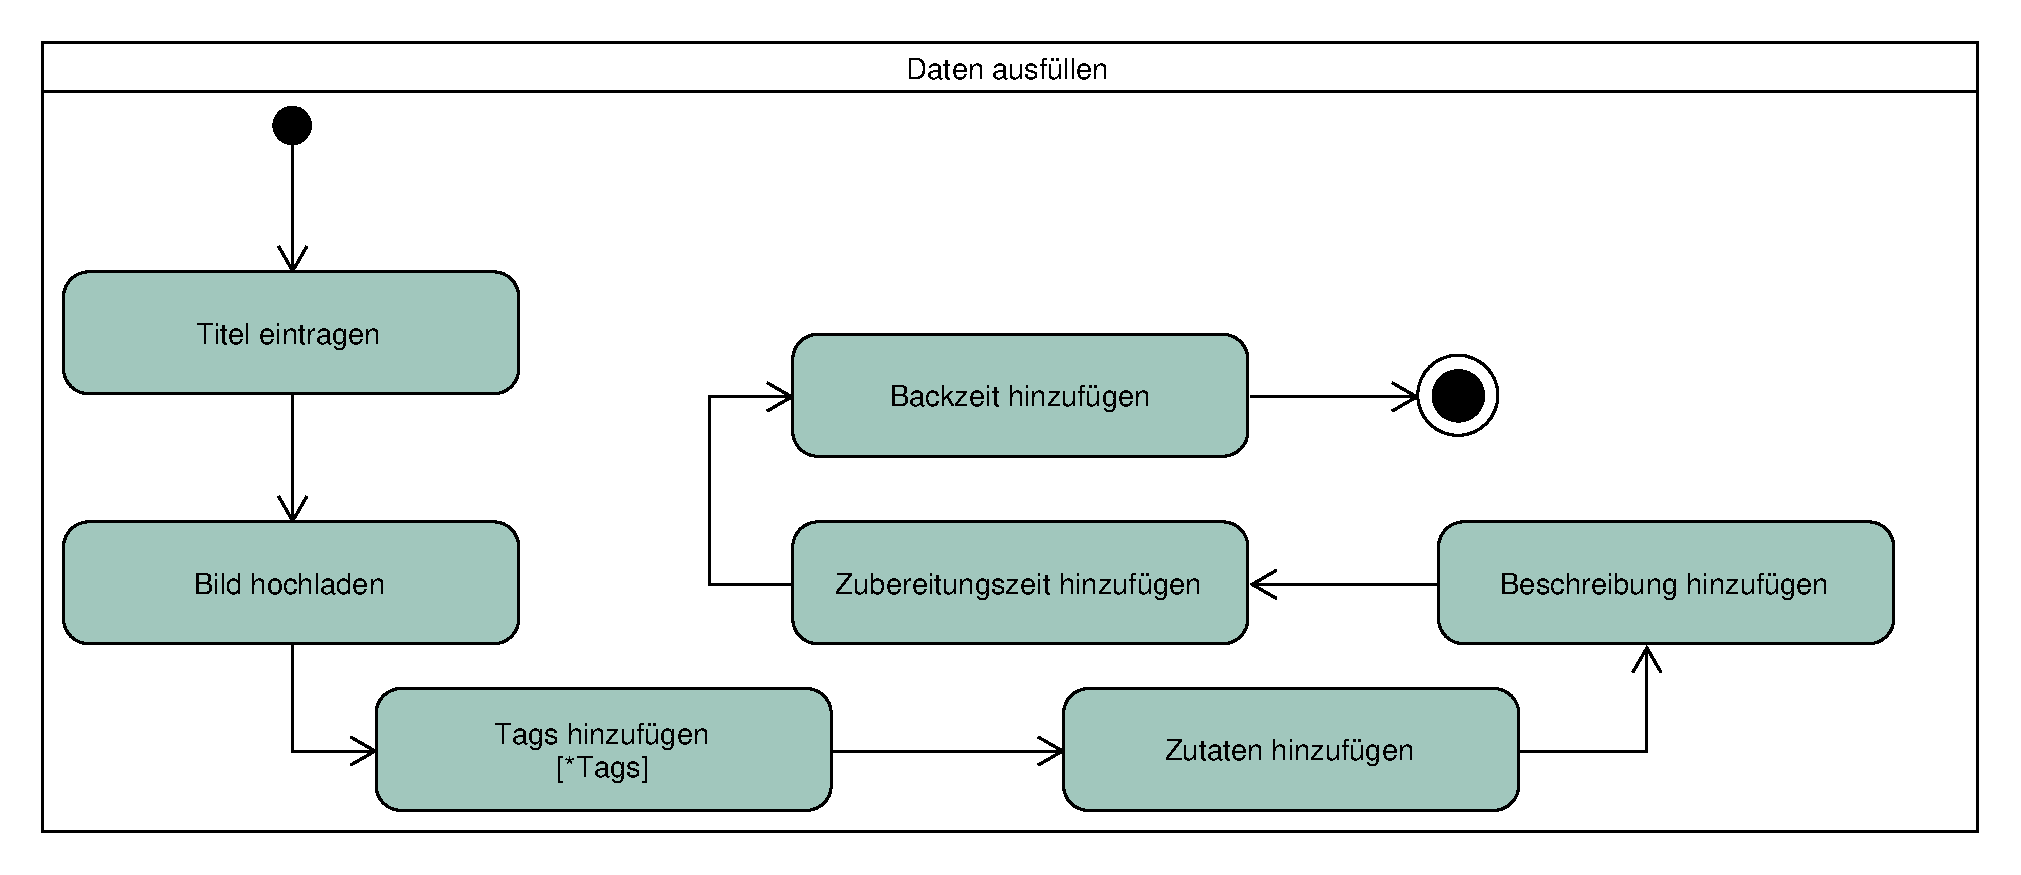
\includegraphics[width=\textwidth]{pics/dynamicDiagram/newAktivitaetsdiagrammRezepterstellenTags.pdf}%
	\caption{Rezept erstellen und veröffentlichen - Tags}%
	\label{diagram}%
\end{figure}

Der Nutzer befindet sich in der Tag erstellen Ansicht. Zuerst wählt er die Funktion ein Tag hinzuzufügen. Daraufhin wählt er aus einen eigenen Tag zu erstellen. Dafür wird ein neuer Tag Eintrag erstellt, den der Nutzer noch einen Namen gibt. Zuletzt speichert er den neu erstellten Tag noch und bestätigt seine Tagliste für das jeweilige Rezept. 


\subsection{Rezept löschen}
\begin{figure}[H]
	\centering
	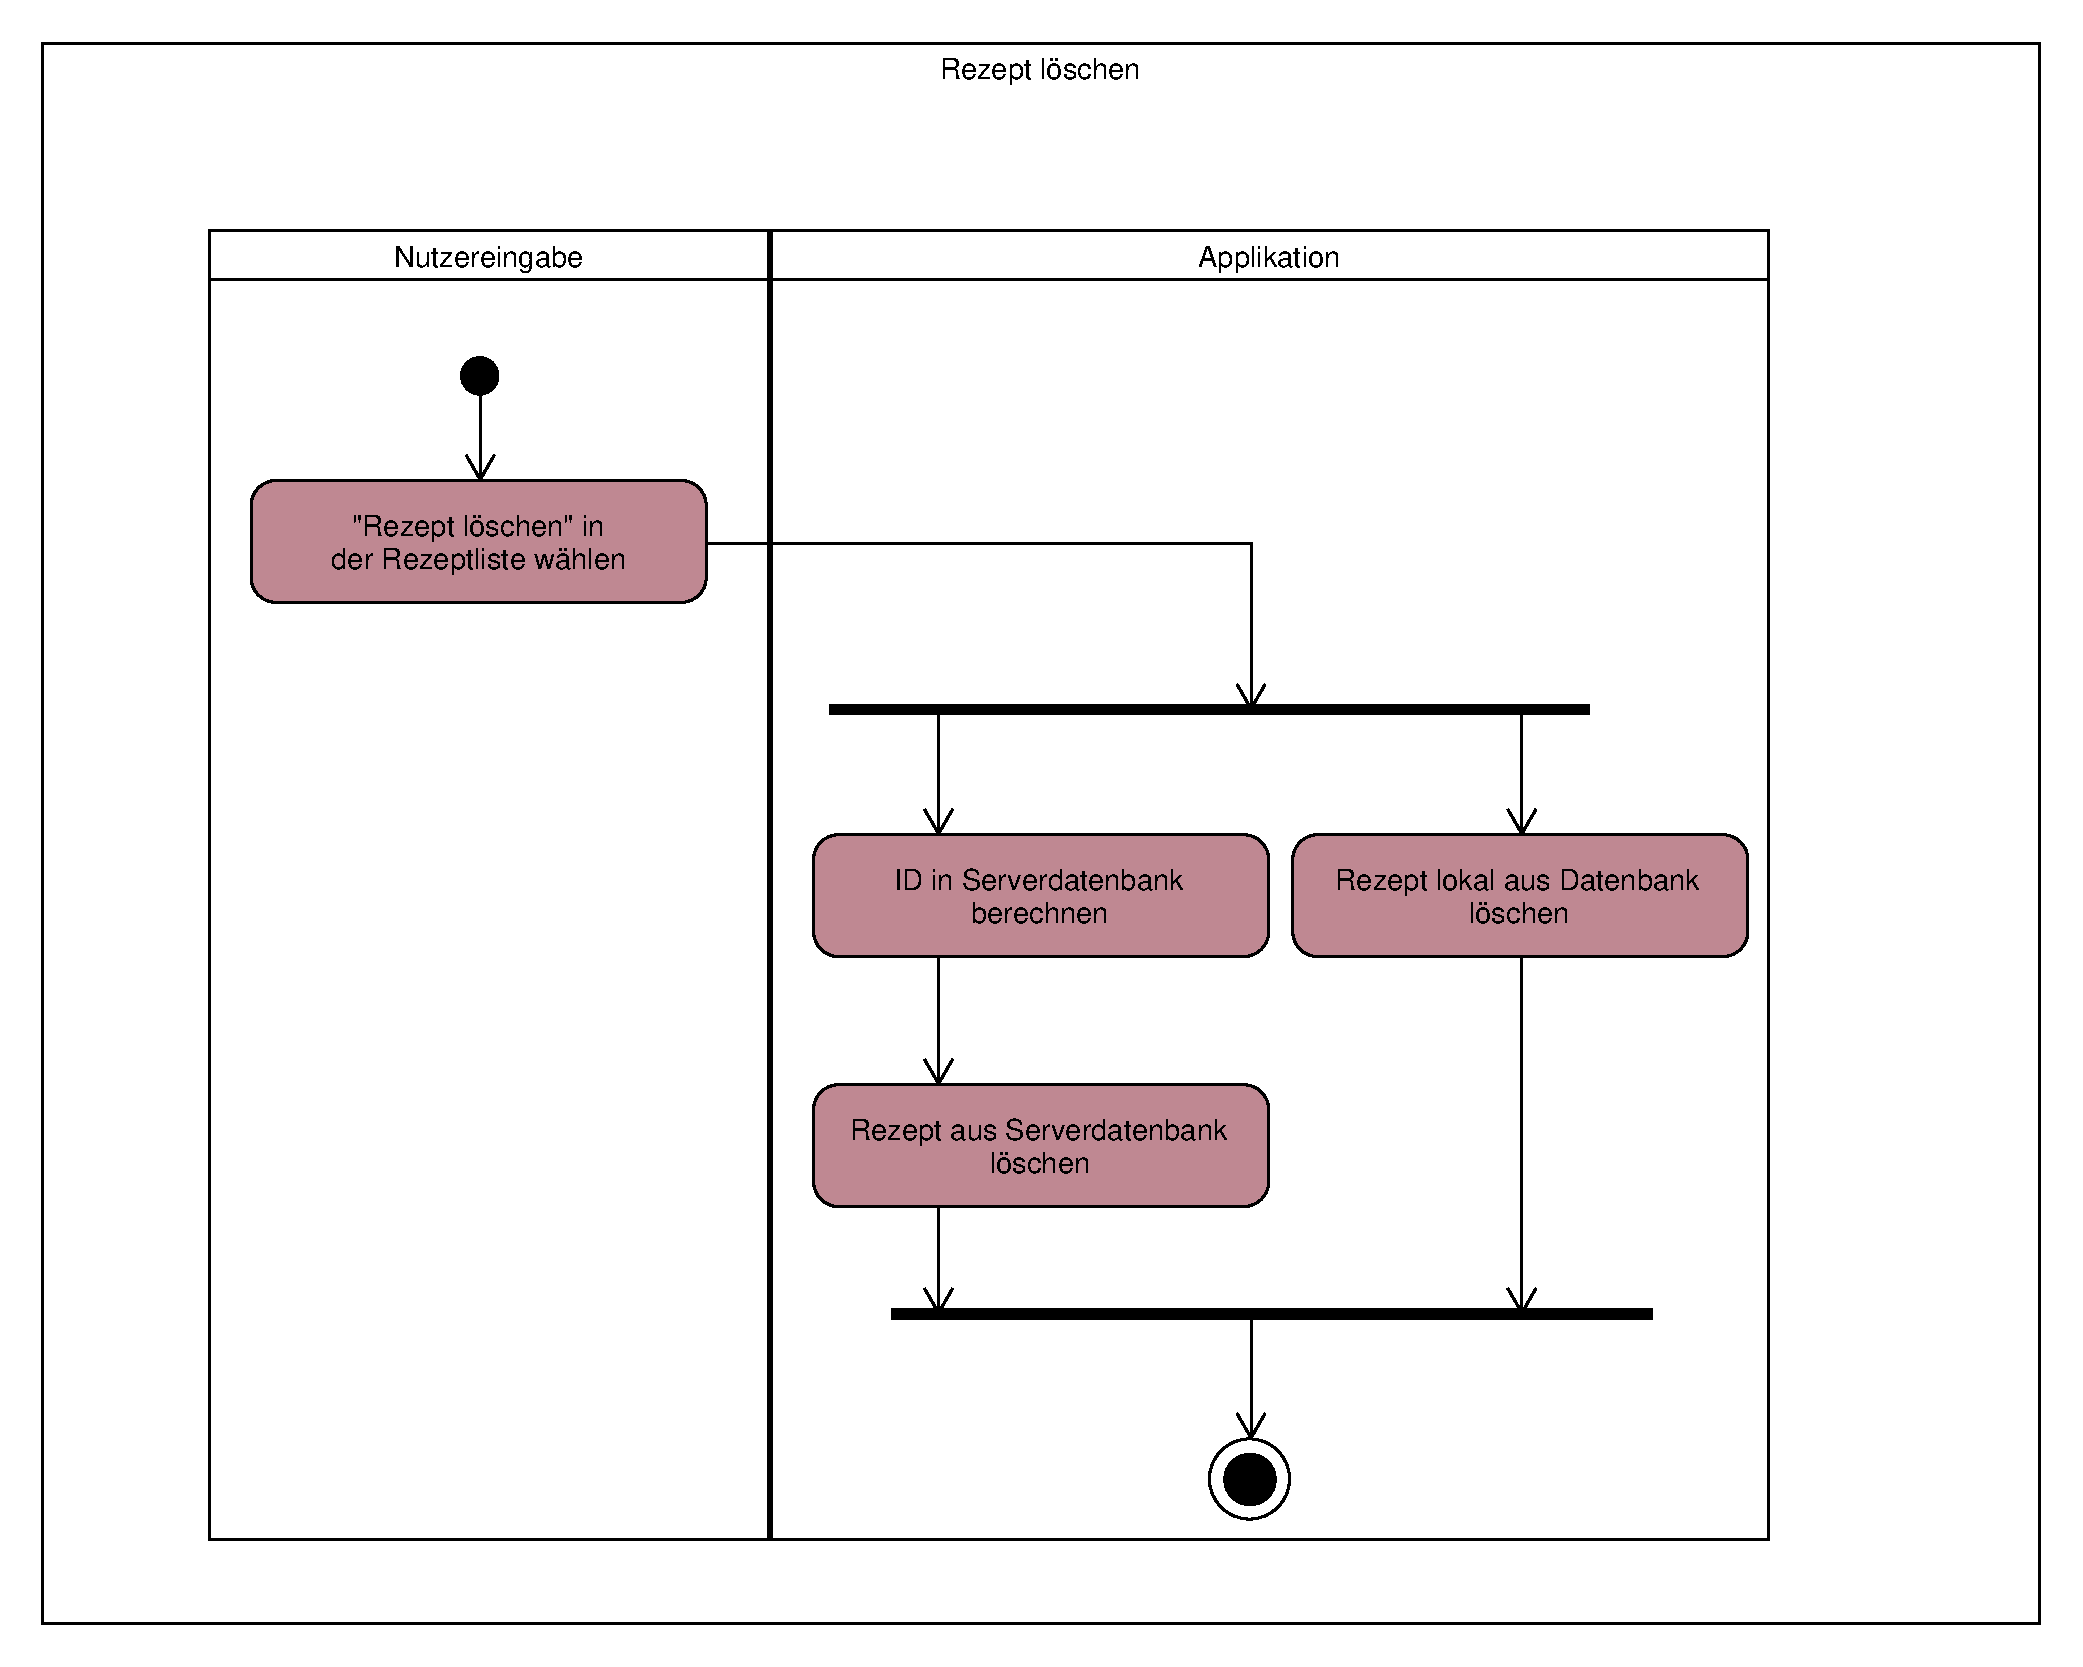
\includegraphics[width=\textwidth]{pics/dynamicDiagram/DeleteRecipeAktivitaetsDiagramm.pdf}%
	\caption{Rezept löschen}%
	\label{diagram}%
\end{figure}

Der Nutzer will ein Rezept entfernen. Dieses kann auch öffentlich sein. Er wählt in der Rezeptliste den Entfernen Button, woraufhin die ID in der Serverdatenbank berechnet wird und das Rezept aus der lokalen Datenbank entfernt wird. Da nach Spezifikation das Rezept auch aus der öffentlichen Datenbank entfernt werden soll, wenn man das private Rezept löscht, wird das Rezept aus der Serverdatenbank gelöscht.
